\documentclass{article}%
\usepackage[T1]{fontenc}%
\usepackage[utf8]{inputenc}%
\usepackage{lmodern}%
\usepackage{textcomp}%
\usepackage{lastpage}%
\usepackage{geometry}%
\geometry{margin=1in}%
\usepackage[utf8]{inputenc}%
\usepackage[titletoc,title]{appendix}%
\usepackage{graphicx,float}%
\usepackage{ragged2e}%
%
\title{\textbf{RELATÓRIO TÉCNICO DE SAÚDE PÚBLICA - SRAG BRASIL}}%
\date{01 de agosto de 2025}%
%
\begin{document}%
\normalsize%
\maketitle%
\section{Análise}%
\label{sec:Anlise}%
\subsection{Geral}%
\label{subsec:Geral}%
Nos últimos meses, o Brasil apresentou uma tendência de redução nos casos de SRAG, com uma diminuição significativa tanto a longo quanto a curto prazo, refletida na queda de casos diários de mais de 2.300 para cerca de 500. Apesar dessa tendência de queda, houve um aumento nos casos entre crianças nas regiões Nordeste e Amazonas, onde o vírus sincicial respiratório (VSR) foi responsável por 42,2\% dos positivos, indicando circulação persistente. Nos últimos 12 meses, os casos totais caíram de 52.407 em maio para 17.125 em dezembro, demonstrando uma redução expressiva na incidência. A taxa de mortalidade também diminuiu de 59.520 óbitos em 2021 para 14.741 em 2025, acompanhada de uma redução na ocupação de UTIs, que passou de 152.558 em 2022 para 56.752 em 2025. A vacinação contra COVID{-}19 e gripe aumentou, chegando a 38.756 vacinados em 2025, contribuindo para a diminuição dos casos e óbitos. Contudo, a circulação contínua de vírus respiratórios reforça a necessidade de estratégias de prevenção e fortalecimento do sistema de saúde, especialmente em regiões vulneráveis.\newline%
%
A taxa de mortalidade por SRAG no Brasil reduziu{-}se significativamente, passando de 59.520 óbitos em 2021 para 14.741 em 2025, indicando melhorias na gestão, tratamento e prevenção. Apesar dessa tendência de queda, o número de casos e óbitos ainda evidencia a importância de ações contínuas de prevenção, sobretudo considerando o aumento de casos entre crianças nas regiões Nordeste e Amazonas, onde o vírus sincicial respiratório (VSR) é predominante. A ocupação de UTIs também diminuiu de 152.558 em 2022 para 56.752 em 2025, refletindo uma possível melhora na capacidade de atendimento hospitalar. Esses dados reforçam a necessidade de manter estratégias de vigilância, vacinação e fortalecimento do sistema de saúde para reduzir ainda mais a mortalidade associada às síndromes respiratórias graves.\newline%
%
A taxa de ocupação de UTIs por pacientes com SRAG no Brasil apresentou uma redução significativa ao longo dos últimos anos, passando de 152.558 internações em 2022 para 56.752 em 2025, indicando uma melhora na capacidade hospitalar e no manejo dos casos graves. Apesar dessa tendência de diminuição, houve um aumento nos casos de SRAG entre crianças nas regiões Nordeste e Amazonas, onde o vírus sincicial respiratório (VSR) foi responsável por 42,2\% dos positivos, reforçando a necessidade de monitoramento contínuo e ações específicas para esses grupos vulneráveis. A diminuição na ocupação de UTIs é um sinal positivo, mas a circulação persistente de vírus respiratórios exige atenção constante para evitar sobrecarga no sistema de saúde.\newline%
%
A taxa de vacinação contra COVID{-}19 e gripe no Brasil tem apresentado crescimento ao longo dos anos, atingindo 38.756 vacinados em 2025, o que representa uma melhora na cobertura vacinal. Apesar do aumento na vacinação, os casos de SRAG continuam a ocorrer, especialmente entre crianças nas regiões Nordeste e Amazonas, onde o vírus sincicial respiratório (VSR) é responsável por uma parcela significativa dos positivos. A maior cobertura vacinal contribui para a redução de casos e óbitos, mas a circulação contínua de vírus respiratórios reforça a necessidade de ações de prevenção, vacinação contínua e fortalecimento do sistema de saúde.\newline%

%
\subsection{Relação Mensal e Anual}%
\label{subsec:RelaoMensaleAnual}%
Nos últimos 30 dias, os casos de SRAG no Brasil apresentaram uma tendência de declínio, com uma redução de casos diários de mais de 2.300 para cerca de 500, indicando uma melhora na situação epidemiológica. Apesar dessa redução geral, houve um aumento nos casos entre crianças nas regiões Nordeste e Amazonas, onde o vírus sincicial respiratório (VSR) foi responsável por aproximadamente 42,2\% dos positivos. Esses dados reforçam a importância de manter estratégias de vigilância, prevenção e ações específicas para grupos vulneráveis, mesmo com a melhora geral na incidência de SRAG.\newline%
%
Ao longo dos últimos 12 meses, o Brasil registrou uma redução significativa nos casos de SRAG, de 52.407 em maio para 17.125 em dezembro, refletindo uma diminuição expressiva na incidência. A taxa de mortalidade também caiu de 59.520 óbitos em 2021 para 14.741 em 2025, acompanhada de uma redução na ocupação de UTIs, que passou de 152.558 em 2022 para 56.752 em 2025. A circulação de vírus como Influenza A (13,9\%) e VSR (44,7\%) permanece, destacando a necessidade de estratégias contínuas de prevenção, vacinação e fortalecimento do sistema de saúde, especialmente em regiões vulneráveis e entre grupos de risco.\newline%
%


\begin{figure}[H]%
\begin{minipage}{0.45\textwidth}%
\centering%
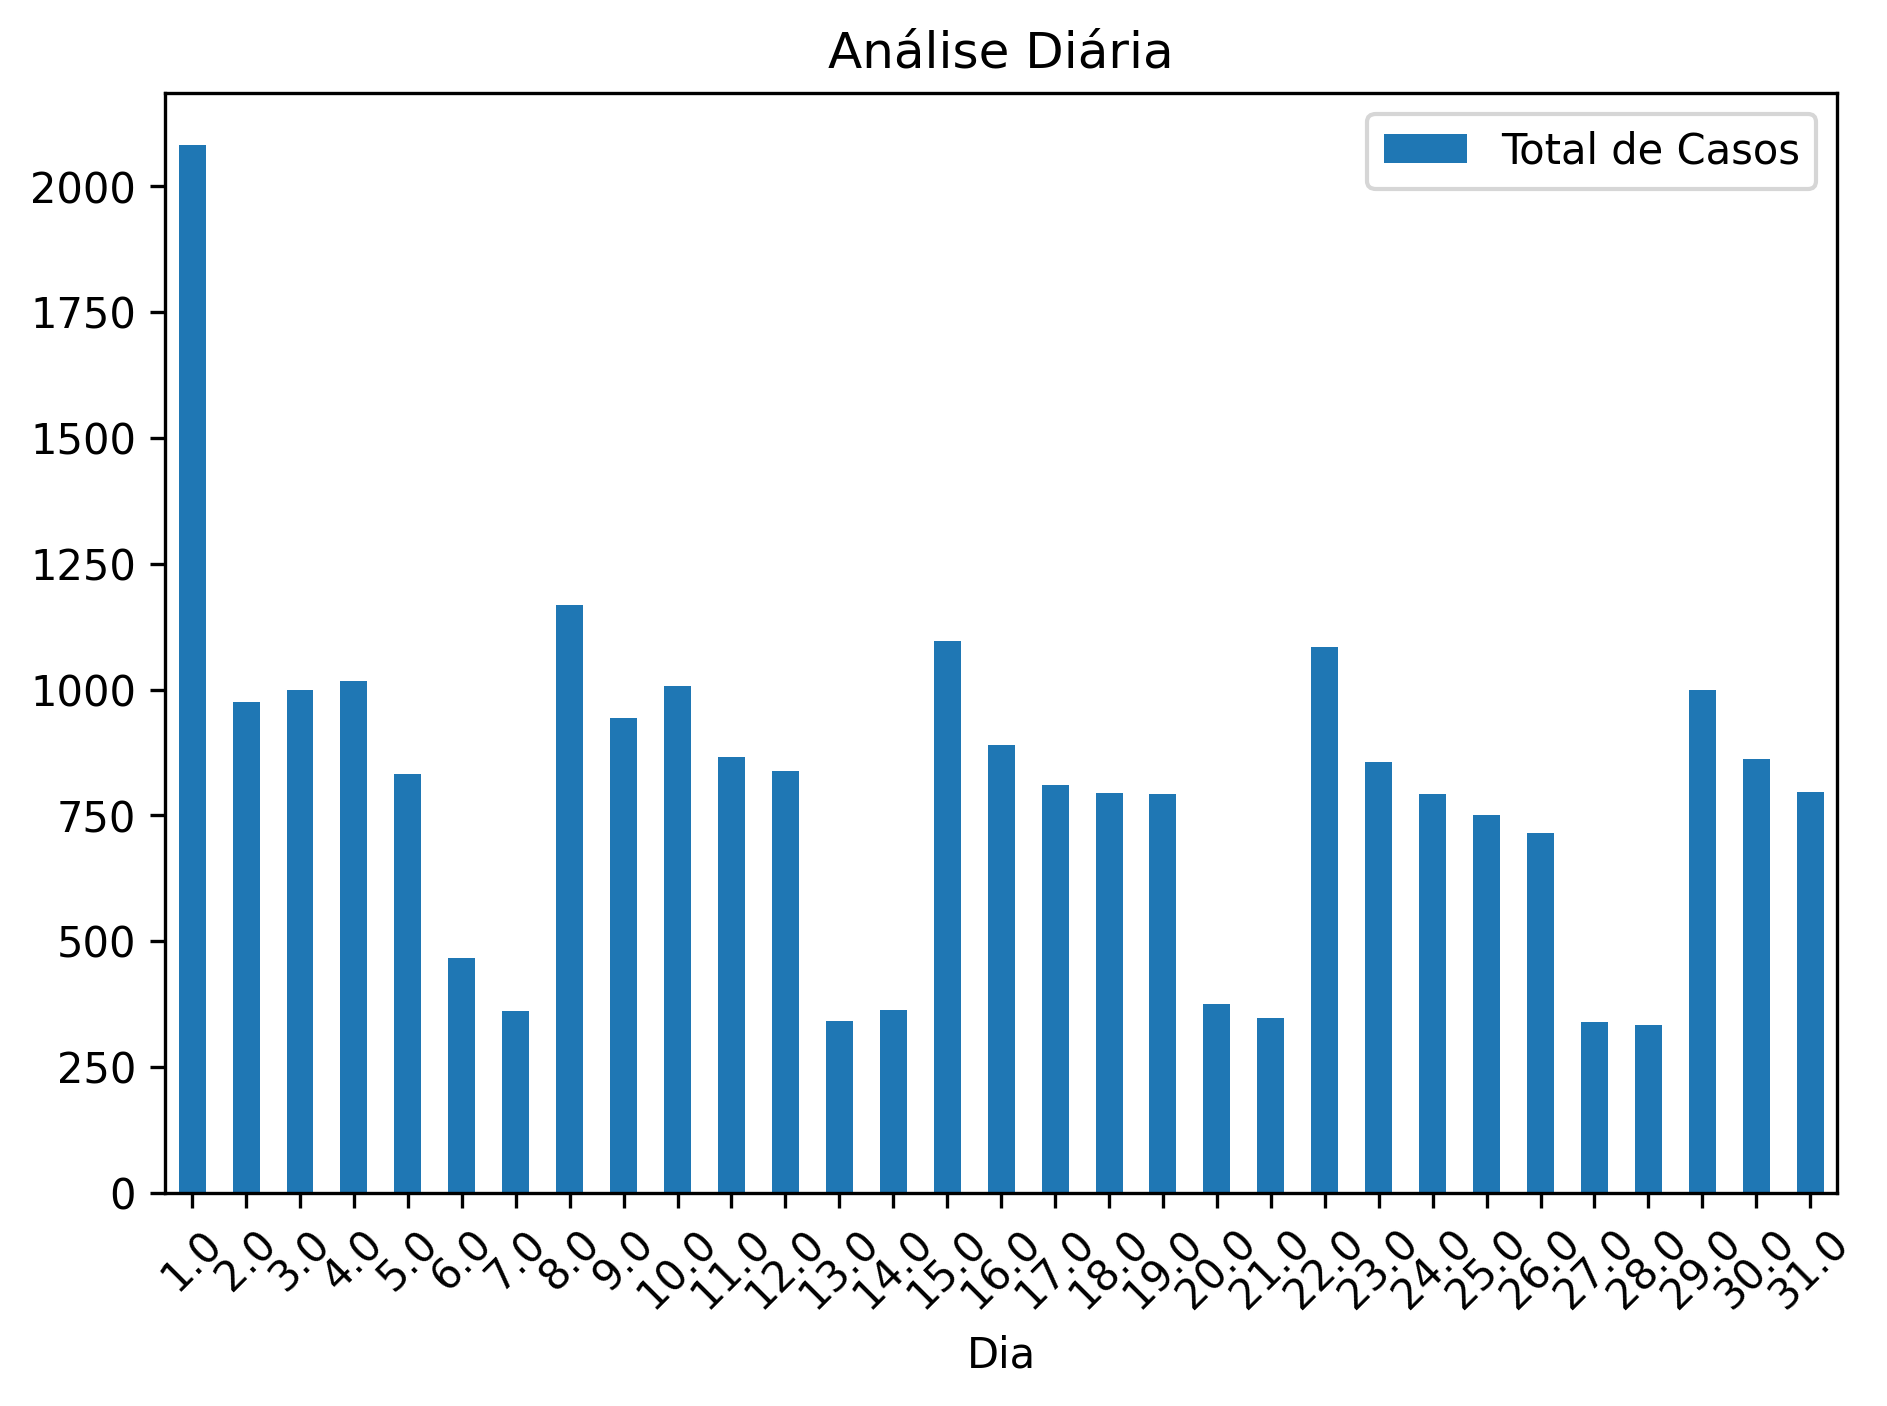
\includegraphics[width=\textwidth]{../graphics/monthly-analysis.png}%
\caption{Análise Mensal}%
\label{fig:casos-30-dias}%
\end{minipage}%
\begin{minipage}{0.45\textwidth}%
\centering%
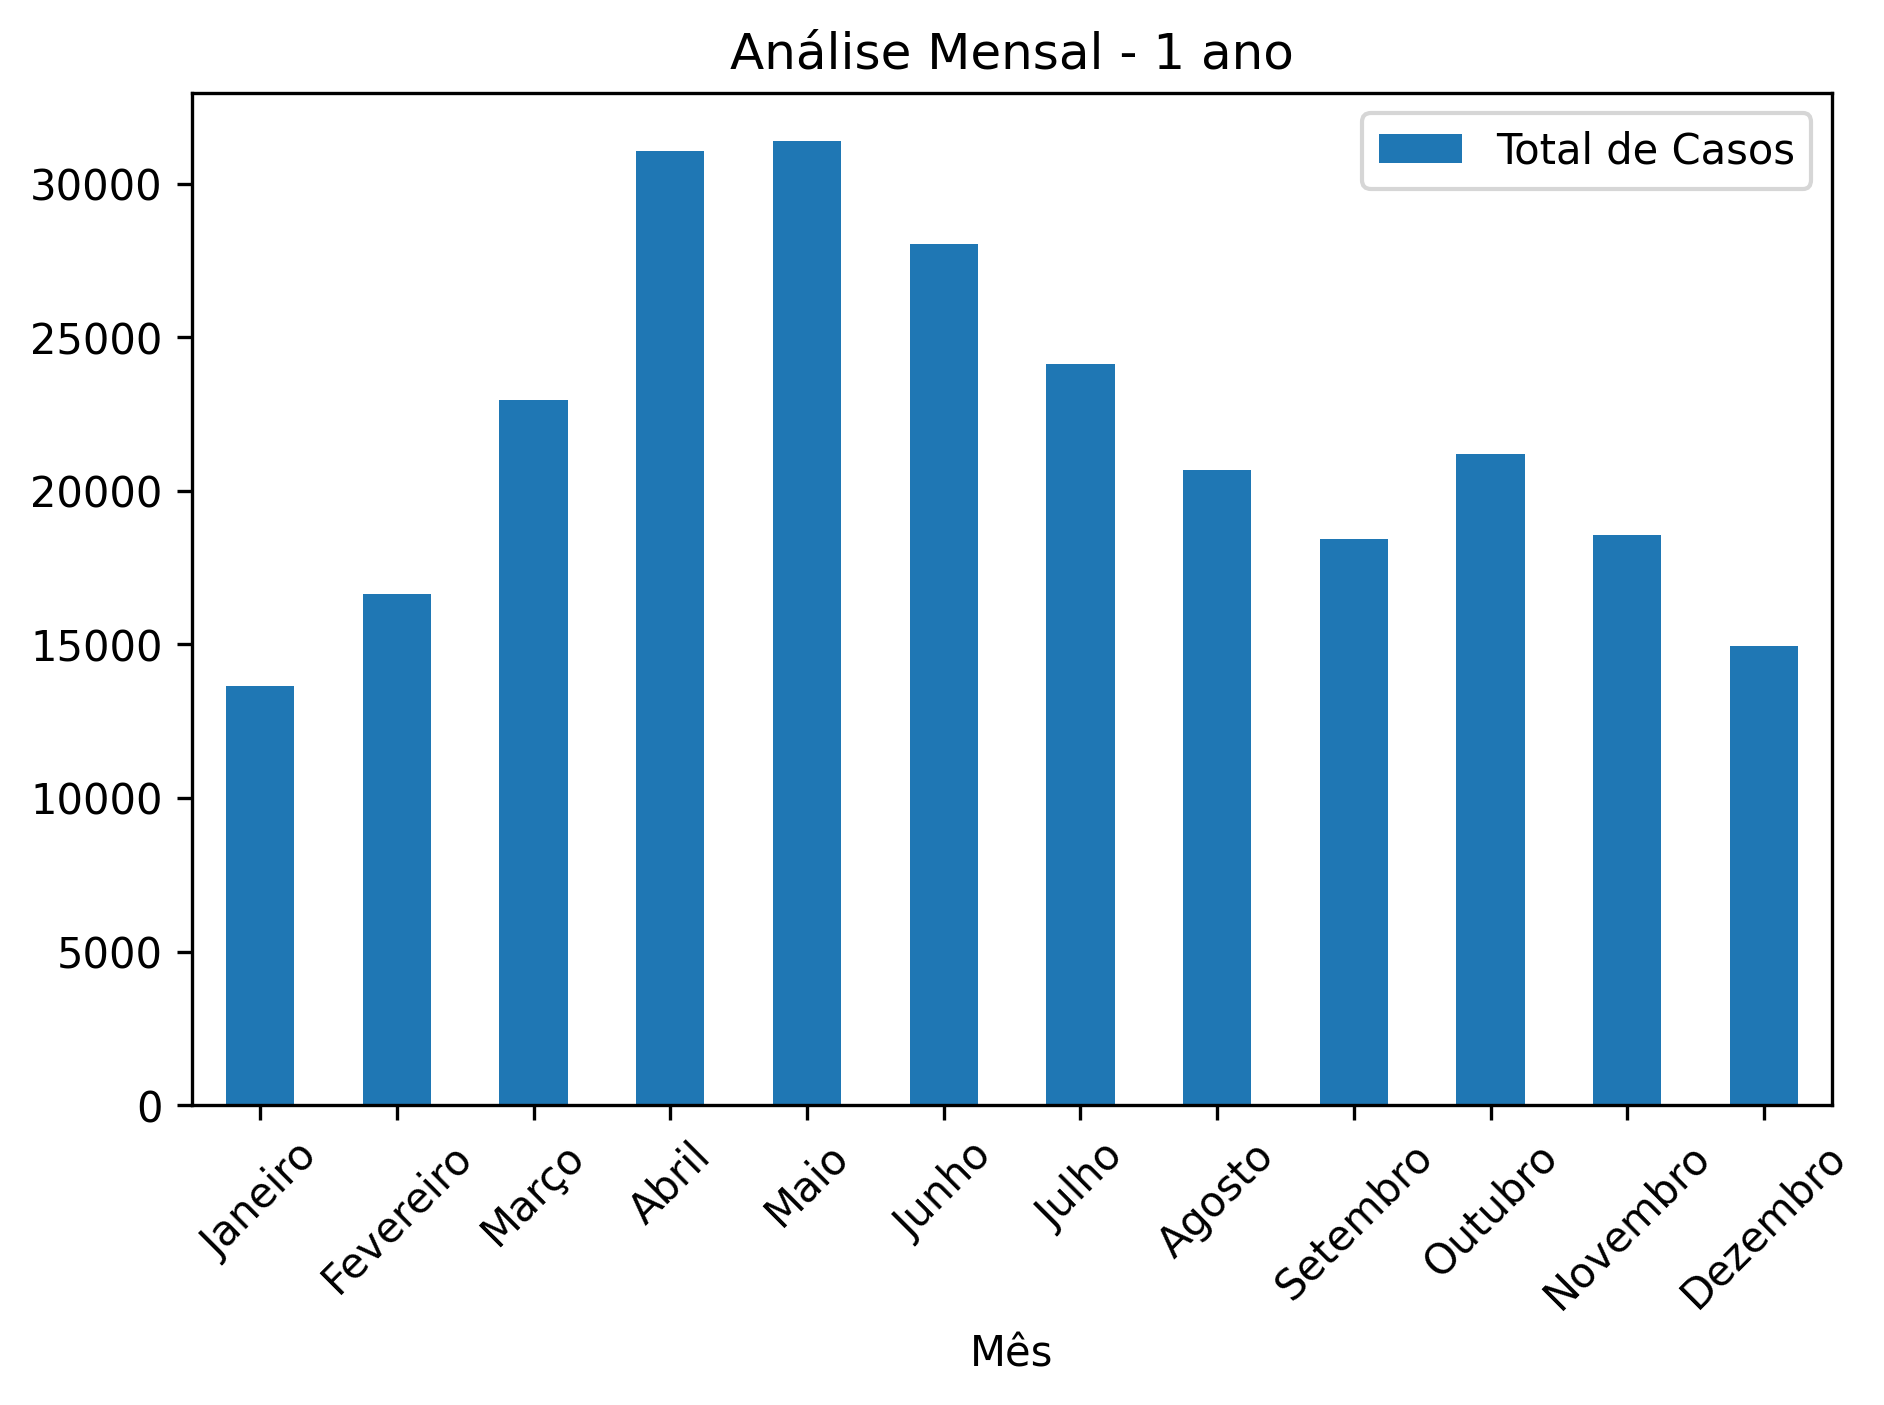
\includegraphics[width=\textwidth]{../graphics/yearly-analysis.png}%
\caption{Análise Anual}%
\label{fig:casos-12-meses}%
\end{minipage}%
\end{figure}

%
\end{document}